%*************************************************

\documentclass[a4paper,10pt]{article}
\usepackage[brazil]{babel}
\usepackage[utf8]{inputenc}
%\usepackage[latin1]{inputenc}
\usepackage{amsthm,amsfonts,amsmath,amssymb}
%img
\usepackage{graphicx}
\usepackage{subfig}
%tabela

%fim
%fim
\usepackage{listings}
\usepackage{makeidx}
\usepackage{enumerate}
\usepackage{hyperref}
\hypersetup{
  colorlinks,
  linkcolor=blue,
  filecolor=blue,
  urlcolor=blue,
  citecolor=blue 
}
%titulo
\title{Servidor Concorrente TCP}
\author{Leandro Kümmel Tria Mendes RA033910 \\ Fernando Teixeira Barros RA085858}
\makeindex
%inicio
\begin{document}
\maketitle
\begin{figure}[!htb]
  \centering
  
\includegraphics[scale=0.5]{logo.jpg}
\end{figure}
\newpage
\tableofcontents
\listoffigures
\listoftables
\newpage
\section{Introdução}
O objetivo desse projeto é implementar um sistema cliente/servidor
concorrente, com operações para o gerenciamento de livros em uma livraria.
Na comunicação entre cliente e servidor utilizou-se o protocolo TCP\footnote{
Mais informações sobre TCP \url{http://www.linktionary.com/t/tcp.html} }, da camada de transporte, e a partir da execução de testes podemos avaliar alguns aspectos
desse protocolo e posteriormente compará-lo com outro(s).
\section{Desenvolvimento}
Linux foi o sistema operacional utilizado para o desenvolvimento (distribuição
2.6.43.8-1.fc15.i686). Igualmente, para os testes utilizou-se duas máquinas com Linux, porém com distribuições diferentes.
\subsection{Protocolo TCP - Transmission Control Protocol}
O protocolo TCP foi escrito de modo a garantir que os dados enviados (pelo
servidor) e recebidos (pelo cliente) de forma correta, na sequência 
adequada e sem erros, pela rede.
\\As características fundamentais do TCP são:
\begin{itemize}
\item \emph{Orientado à conexão}: necessidade de uma conexão.
\item \emph{Ponto a ponto}: conexão é estabelecida entre dois pontos.
\item \emph{Confiabilidade}: Permite a recuperação de arquivos perdidos, elimina 
arquivos duplicados, recupera dados corrompidos, entrega na ordem do envio e 
pode recuperar o ``link'' entre cliente e servidor, caso esse, por algum motivo,
seja perdido.
\item \emph{Full duplex}: Possível transferência simultânea, entre cliente e 
servidor.
\item \emph{Handshake}: Mecanismo de estabelecimento e finalização de conexão.
O TCP garante que, no final da conexão, \textbf{todos} os pacotes sejam 
entregues ou recebidos.
\item \emph{Entrega ordenada}: A aplicação entrega ao TCP blocos de dados de 
tamanho variável. Esse protocolo divide estes dados em segmentos de tamanho 
especificado (valor MTU). Sabe-se que camadas inferiores à de transporte podem 
fazer com que os pacotes não cheguem na ordem em que foram enviados. Porém, o TCP
garante a reconstrução dos segmentos no cliente (TCP utiliza um número de 
sequência).
\item \emph{Controle de fluxo}: O protocolo em estudo utiliza-se de um campo 
denominado \textbf{janela} para controlar o fluxo
\end{itemize}
\subsection{Implementação}
O projeto conta com cinco diretórios, cada um com seu Makefile (exceto relatorio e estat), arquivos
principal (main.c e main.h) e um README.md\footnote{Leia esse arquivo antes de
executar o sistema} para instruções adicionais. Há também um Makefile no diretório raiz, o qual 
compila todo o sistema.
\\Os diretório são:
\begin{enumerate}[I.]
\label{sec:dirs}
\item \label{itm:common} \emph{common}: Contém arquivos de uso comum, tanto pelo servidor quanto 
pelo cliente, inclusive o arquivo que calcula a média dos testes executados.
\item \label{itm:server} \emph{server}: Contém os arquivos que preparam uma porta para esperar
conexões e manipulam o sistema de livraria.
\item \label{itm:client} \emph{client}: Funções que provém conexão com um servidor, envio das opções
escolhidas pelo cliente e interface para as respostas do sistema de livraria
(servidor).
\item \label{itm:estat} \emph{estat}: Medidas de tempo efetuadas pelo teste.
\item \label{itm:relatorio} \emph{relatorio}: Arquivos de criação do relatório em LaTeX.
\end{enumerate}
\subsubsection{Manipulação de dados}
Todas as estruturas utilizadas para leitura/escrita dos livros são dinâmicas. 
\\Arquivos presentes no diretório \emph{common}[\ref{itm:common}]:
\begin{enumerate}[I.]
\item \emph{error.c[\ref{itm:error.c}] error.h}: Gerencia erros que eventualmente podem ocorrer.
\item \emph{common.c[\ref{itm:common.c}] common.h}: Funções de uso comum.
\item \label{itm:avl} \emph{avl.c[\ref{itm:avl.c}] avl.h}: Gerencia a estrutura básica da livraria, utiliza-se 
árvore AVL\footnote{ \url{http://pages.cs.wisc.edu/~ealexand/cs367/NOTES/AVL-Trees/index.html} }, pois a busca, 
inserção/atualização têm complexidade \boxed{O(logN)} , sendo N
o número de elementos na árvore, no caso a quantidade de livros diferentes.
\item \emph{archives.c[\ref{itm:archives.c}] archives.h}: Manipula arquivos. Faz a leitura do arquivo
da livraria\footnote{Ver README.md para mais detalhes do arquivo da livraria}.
\item \label{itm:tcp} \emph{tcp.c[\ref{itm:tcp.c}] tcp.h}: Contém apenas algumas constantes.
\item \emph{books.c books.h}: Gerencia a estrutura básica de um livro e seus autores.
\item \label{itm:tempo}\emph{tempo.c[\ref{itm:tempo.c}] tempo.h}: Gerencia a estrutura de testes, lê e escreve em arquivos localizados no diretório \emph{estat}[\ref{itm:estat}].
\item \emph{livros/livros}: Arquivo contendo os livros\footnote{Ver README.md para mais detalhes do arquivo da livraria}.
\end{enumerate}
\subsubsection{Conexão Servidor/Cliente}
Compreende dois diretórios \emph{server}[\ref{itm:server}] e \emph{client}[\ref{itm:client}]
\\\textbf{Servidor}:
\begin{enumerate}[I.] \item \emph{server.c[\ref{itm:server.c}] server.h}: Apenas inicia o servidor
dada um número de uma porta.
\item \label{itm:tcpserver} \emph{tcp\_server.c[\ref{itm:tcp_server.c}] tcp\_server.h}: Gerencia tanto
as conexões com os clientes quanto a comunicação, em outras palavras, o
tcp\_server.c recebe um stream do tcp\_client.c[\ref{itm:tcpclient}] e envia uma
resposta adequada ao mesmo.
\item \emph{login.c[\ref{itm:login.c}] login.h}: Gerencia o login necessário para editar a
quantidade de um livro.
\end{enumerate}
\textbf{Cliente}:
\begin{enumerate}[I.]
\item \emph{client.c client.h}: Apenas inicia a comunicação com um servidor dado o endereço IP e um número de uma porta.
\item \label{itm:tcpclient} \emph{tcp\_client.c tcp\_client.h}: Gerencia tanto 
a criação de uma conexão entre o cliente e servidor quanto a leitura, da entrada dada pelo usuário do sistema, e a comunicação entre hospedeiro e cliente.
\end{enumerate}
\subsection{Coleta e gerência de dados para testes}
Para realizar os testes implementou-se alguns arquivos adicionas[\ref{itm:tempo}]. Uma constante, denominada NUM\_TESTES\footnote{Nesse sistema consideramos NUM\_TESTES igual a 100} , contém o número de testes a serem realizados, ou seja, cada opção do \emph{menu}[\ref{itm:tcpserver}] é executada NUM\_TESTE vezes. Todos os dados são 
salvos no diretório \emph{estat}[\ref{itm:estat}].
\subsection{Vantagens da implementação}
O sistema de livraria é um sistema robusto e com baixa complexidade de tempo.
A escolha da estrutura de árvore \textit{AVL}[\ref{itm:avl}], possibilitou em boa 
performance em questão de tempo de processamento, uma vez que, essa estrutura
mostrou-se eficaz para o problema e possui melhor complexidade de tempo com 
relação a outras estruturas, além da implementação e manutenção serem relativamente	
simples.
\\ Com relação às conexões e comunicações entre cliente/servidor, vale ressaltar
que há uma troca de mensagens\footnote{Sabe-se que o TCP envia/recebe streams}
inicial entre os dois, na qual o conteúdo do stream é o número de bytes da maior
mensagem possível a ser enviada pelo servidor.
Como a função \boxed{rcv(int sockfd, void *buf, size_t len, int
flags)}\footnote{\url{http://linux.die.net/man/2/recv}} começa a ler o buffer, o
qual é escrito o stream enviado pelo servidor, antes do mesmo estar com ele
completo, em outras palavras, antes de toda mensagem enviada pelo servidor estar
escrita no buffer então, o número de bytes das mensagens mostra-se necessário,
uma vez que, podemos controlar a função \boxed{rcv(int sockfd, void *buf, size_t
len, int flags)}, junto ao envio de mensagens de controle (ACK\footnote{Veja
tcp.h[\ref{itm:tcp}]}), afim de ler o buffer apenas quando o mesmo estiver
completo.\footnote{The receive calls normally return any data available, up to
the requested amount, rather than waiting for receipt of the full amount
requested.} \begin{figure}[!htb]
  \centering
  \subfloat[Fluxograma Servidor]{
  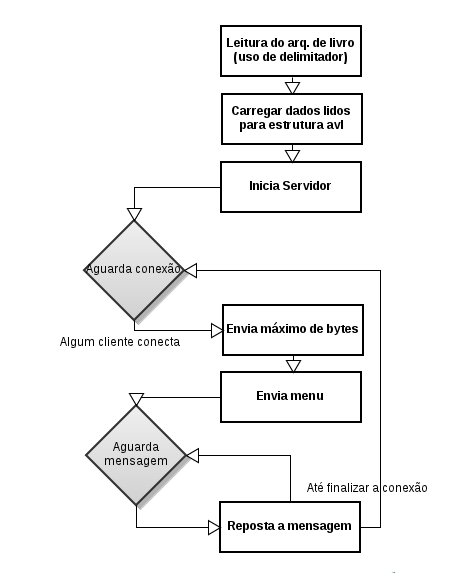
\includegraphics[width=150px,height=300px]{fluxo_servidor.png}
  \label{fluxoservidor}
  }
  \quad %espaco separador
   \subfloat[Fluxograma Cliente]{
     \label{fluxoserver}
     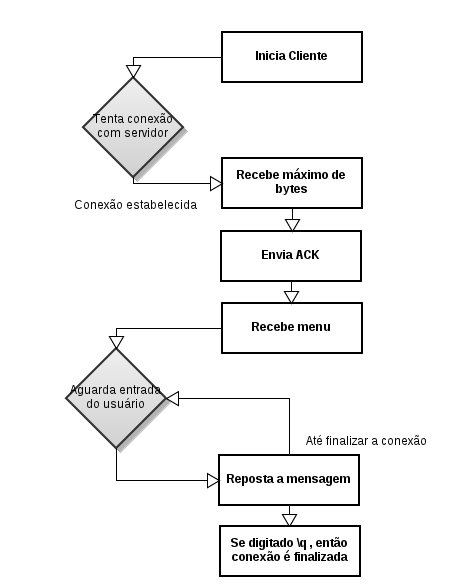
\includegraphics[width=150px,height=300px]{fluxo_cliente.png}
   }
   \caption{Fluxogramas}
   \label{figfluxos}
\end{figure}
\begin{figure}[!htb]
  \centering
  \label{fluxotempo}
  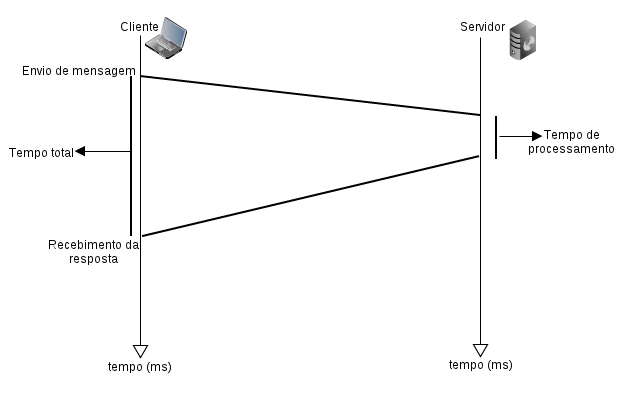
\includegraphics[scale=0.5]{fluxo_tempo.png}
  \caption{Definição do cálculo dos tempos}
\end{figure}
\newpage
\section{Resultados e discussões}
Os testes foram efetuados em duas máquinas, ambas conectadas à rede porém, não localmente. Denominaremos a máquina servidor como [S] e a cliente como [C]. [S] e [C] estão em continentes diferentes.
\\Foram efetuadas 100 medições para cada opção do menu[\ref{itm:tcpserver}], ao todo foram 600 medições de tempo. Dividiu-se o tempo em tempo de processamento e tempo de comunicação, sendo o último a diferença entre o tempo total e o tempo de processamento.
\subsection{Tabelas e gráficos}
\subsubsection{Tempo total}
Representaremos todas as 100 medidas de tempo total das 6 opções do menu[\ref{itm:tcpserver}]
\addtolength{\abovecaptionskip}{-8pt}
\begin{table}
  \tiny
  \centering
  \begin{tabular}{|c|}
    \hline
    Opção 1 [ms] \\
    \hline
    186134.000000\\
187389.000000\\
187232.000000\\
186872.000000\\
184125.000000\\
186449.000000\\
186252.000000\\
189478.000000\\
183976.000000\\
208636.000000\\
201516.000000\\
208826.000000\\
199975.000000\\
187522.000000\\
187232.000000\\
186570.000000\\
184801.000000\\
187593.000000\\
187224.000000\\
199953.000000\\
184321.000000\\
184627.000000\\
185264.000000\\
182234.000000\\
185997.000000\\
183630.000000\\
195198.000000\\
185220.000000\\
184872.000000\\
184440.000000\\
215691.000000\\
185690.000000\\
185212.000000\\
184893.000000\\
184262.000000\\
187784.000000\\
190727.000000\\
186847.000000\\
187853.000000\\
187898.000000\\
184341.000000\\
192566.000000\\
192088.000000\\
195817.000000\\
189500.000000\\
187443.000000\\
197499.000000\\
188974.000000\\
187302.000000\\
187996.000000\\
207983.000000\\
183661.000000\\
188076.000000\\
193033.000000\\
203251.000000\\
191111.000000\\
208720.000000\\
191228.000000\\
208735.000000\\
192248.000000\\
188302.000000\\
199366.000000\\
185200.000000\\
189354.000000\\
184946.000000\\
212453.000000\\
186990.000000\\
187158.000000\\
186925.000000\\
187869.000000\\
190985.000000\\
192168.000000\\
188490.000000\\
198904.000000\\
211250.000000\\
190856.000000\\
186611.000000\\
184224.000000\\
188581.000000\\
200660.000000\\
187730.000000\\
183613.000000\\
182749.000000\\
184443.000000\\
191332.000000\\
186974.000000\\
183429.000000\\
188809.000000\\
187492.000000\\
189442.000000\\
188319.000000\\
212336.000000\\
184941.000000\\
199550.000000\\
188052.000000\\
184290.000000\\
189488.000000\\
187303.000000\\
187554.000000\\
184799.000000\\
    
    \hline
  \end{tabular}
  \begin{tabular}{|c|}
    \hline
    Opção 2 [ms] \\
    \hline
    379959.000000\\
375949.000000\\
370050.000000\\
376848.000000\\
371970.000000\\
378102.000000\\
384827.000000\\
389313.000000\\
383991.000000\\
405586.000000\\
412777.000000\\
391916.000000\\
396349.000000\\
372619.000000\\
388165.000000\\
385603.000000\\
371246.000000\\
390852.000000\\
372110.000000\\
374939.000000\\
372986.000000\\
372867.000000\\
386347.000000\\
380072.000000\\
374853.000000\\
392627.000000\\
374530.000000\\
407452.000000\\
370111.000000\\
371786.000000\\
383864.000000\\
380330.000000\\
412519.000000\\
379579.000000\\
379550.000000\\
374553.000000\\
381625.000000\\
372065.000000\\
382966.000000\\
387376.000000\\
375648.000000\\
379688.000000\\
375459.000000\\
376471.000000\\
375927.000000\\
392176.000000\\
383317.000000\\
386863.000000\\
377841.000000\\
411911.000000\\
394753.000000\\
372805.000000\\
384455.000000\\
376016.000000\\
377246.000000\\
381236.000000\\
406373.000000\\
381707.000000\\
405468.000000\\
377373.000000\\
377298.000000\\
373149.000000\\
374735.000000\\
376027.000000\\
388418.000000\\
375709.000000\\
368840.000000\\
388926.000000\\
368673.000000\\
371949.000000\\
376248.000000\\
414355.000000\\
379056.000000\\
376609.000000\\
401945.000000\\
397610.000000\\
386879.000000\\
400721.000000\\
374753.000000\\
371650.000000\\
370857.000000\\
367969.000000\\
369355.000000\\
372903.000000\\
370708.000000\\
370738.000000\\
381375.000000\\
383981.000000\\
380894.000000\\
385549.000000\\
386792.000000\\
382847.000000\\
374897.000000\\
383519.000000\\
384007.000000\\
367800.000000\\
372088.000000\\
375202.000000\\
375090.000000\\
376349.000000\\

    \hline
  \end{tabular}
  \begin{tabular}{|c|}
    \hline
    Opção 3 [ms] \\
    \hline
    376944.000000\\
400865.000000\\
370365.000000\\
378147.000000\\
383610.000000\\
372725.000000\\
406249.000000\\
385968.000000\\
399733.000000\\
395936.000000\\
410493.000000\\
376920.000000\\
372669.000000\\
386818.000000\\
396910.000000\\
387320.000000\\
370559.000000\\
369696.000000\\
388092.000000\\
380271.000000\\
383898.000000\\
385548.000000\\
370293.000000\\
372772.000000\\
374805.000000\\
371155.000000\\
372819.000000\\
376015.000000\\
369152.000000\\
384647.000000\\
379819.000000\\
387667.000000\\
393443.000000\\
374329.000000\\
368171.000000\\
387358.000000\\
388207.000000\\
382376.000000\\
374341.000000\\
372352.000000\\
376884.000000\\
379830.000000\\
376261.000000\\
378325.000000\\
375789.000000\\
390918.000000\\
375919.000000\\
375807.000000\\
373075.000000\\
398038.000000\\
414173.000000\\
375157.000000\\
383204.000000\\
390993.000000\\
371334.000000\\
426817.000000\\
411600.000000\\
389590.000000\\
404575.000000\\
374398.000000\\
375974.000000\\
368093.000000\\
368255.000000\\
372728.000000\\
375615.000000\\
389035.000000\\
395126.000000\\
387413.000000\\
370925.000000\\
371555.000000\\
428680.000000\\
372998.000000\\
375593.000000\\
374853.000000\\
369829.000000\\
372959.000000\\
383926.000000\\
374829.000000\\
373974.000000\\
379977.000000\\
394231.000000\\
371856.000000\\
373896.000000\\
379262.000000\\
388287.000000\\
381855.000000\\
402648.000000\\
382801.000000\\
380474.000000\\
403718.000000\\
367633.000000\\
385087.000000\\
380782.000000\\
419549.000000\\
376016.000000\\
372644.000000\\
387662.000000\\
368928.000000\\
424597.000000\\
375084.000000\\

    \hline
  \end{tabular}
  \begin{tabular}{|c|}
    \hline
    Opção 4 [ms] \\
    \hline
    387384.000000\\
374474.000000\\
427843.000000\\
382172.000000\\
378222.000000\\
376055.000000\\
376315.000000\\
194417.000000\\
380161.000000\\
379678.000000\\
405222.000000\\
388630.000000\\
378038.000000\\
372268.000000\\
382632.000000\\
197574.000000\\
580704.000000\\
380162.000000\\
404885.000000\\
385934.000000\\
377787.000000\\
381415.000000\\
648557.000000\\
374264.000000\\
388695.000000\\
384329.000000\\
207618.000000\\
379876.000000\\
376061.000000\\
213692.000000\\
376815.000000\\
226705.000000\\
219818.000000\\
557030.000000\\
373069.000000\\
382635.000000\\
382833.000000\\
384977.000000\\
383732.000000\\
391522.000000\\
207540.000000\\
574534.000000\\
375237.000000\\
195837.000000\\
600420.000000\\
377294.000000\\
195515.000000\\
378985.000000\\
379188.000000\\
208805.000000\\
570363.000000\\
372253.000000\\
211366.000000\\
388508.000000\\
392704.000000\\
495126.000000\\
407102.000000\\
211494.000000\\
384187.000000\\
382093.000000\\
211832.000000\\
372351.000000\\
375555.000000\\
572923.000000\\
386961.000000\\
386677.000000\\
392726.000000\\
380430.000000\\
384439.000000\\
604662.000000\\
389692.000000\\
398815.000000\\
562676.000000\\
372192.000000\\
375258.000000\\
196175.000000\\
418567.000000\\
372079.000000\\
194860.000000\\
422544.000000\\
377544.000000\\
374463.000000\\
376970.000000\\
376326.000000\\
400862.000000\\
391890.000000\\
206752.000000\\
412661.000000\\
390881.000000\\
223366.000000\\
373351.000000\\
400206.000000\\
575655.000000\\
388674.000000\\
383672.000000\\
198639.000000\\
377000.000000\\
372877.000000\\
387913.000000\\
435362.000000\\

    \hline
  \end{tabular}
  \begin{tabular}{|c|}
    \hline
    Opção 5 [ms] \\
    \hline
    825847.000000\\
790328.000000\\
756741.000000\\
751569.000000\\
803135.000000\\
790978.000000\\
765067.000000\\
969968.000000\\
817787.000000\\
781436.000000\\
823250.000000\\
783629.000000\\
775647.000000\\
753483.000000\\
746090.000000\\
989000.000000\\
777143.000000\\
791327.000000\\
747343.000000\\
789833.000000\\
766127.000000\\
789028.000000\\
973036.000000\\
742324.000000\\
795654.000000\\
780909.000000\\
954986.000000\\
775651.000000\\
784223.000000\\
954416.000000\\
752007.000000\\
978050.000000\\
974375.000000\\
784645.000000\\
806536.000000\\
818931.000000\\
809578.000000\\
800117.000000\\
763441.000000\\
791098.000000\\
999633.000000\\
759718.000000\\
778494.000000\\
973809.000000\\
748282.000000\\
763193.000000\\
973658.000000\\
780145.000000\\
815248.000000\\
1031502.000000\\
758345.000000\\
775336.000000\\
967862.000000\\
792555.000000\\
797030.000000\\
823025.000000\\
772950.000000\\
1006556.000000\\
747142.000000\\
786838.000000\\
963735.000000\\
787738.000000\\
818610.000000\\
768839.000000\\
791648.000000\\
795321.000000\\
796099.000000\\
798079.000000\\
799194.000000\\
749932.000000\\
812855.000000\\
785395.000000\\
773942.000000\\
780995.000000\\
838770.000000\\
990778.000000\\
740847.000000\\
780270.000000\\
964569.000000\\
781779.000000\\
801518.000000\\
798388.000000\\
830862.000000\\
791705.000000\\
796368.000000\\
804335.000000\\
965144.000000\\
755087.000000\\
785804.000000\\
967479.000000\\
803788.000000\\
797278.000000\\
743384.000000\\
772949.000000\\
795339.000000\\
958940.000000\\
763934.000000\\
787705.000000\\
812114.000000\\
755337.000000\\

    \hline
  \end{tabular}
  \begin{tabular}{|c|}
    \hline
    Opção 6 [ms] \\
    \hline
    399407.000000\\
373987.000000\\
377698.000000\\
390804.000000\\
370656.000000\\
397889.000000\\
371087.000000\\
375421.000000\\
405330.000000\\
391226.000000\\
405368.000000\\
375988.000000\\
399652.000000\\
379150.000000\\
386807.000000\\
374798.000000\\
371615.000000\\
374636.000000\\
368790.000000\\
377796.000000\\
378929.000000\\
401560.000000\\
373652.000000\\
375463.000000\\
383348.000000\\
393012.000000\\
375117.000000\\
371329.000000\\
379558.000000\\
371527.000000\\
372939.000000\\
389300.000000\\
382385.000000\\
373910.000000\\
396343.000000\\
384945.000000\\
372323.000000\\
374682.000000\\
390692.000000\\
373671.000000\\
382487.000000\\
380988.000000\\
397173.000000\\
369877.000000\\
370903.000000\\
384424.000000\\
396167.000000\\
371593.000000\\
379885.000000\\
411339.000000\\
373207.000000\\
368434.000000\\
371541.000000\\
374001.000000\\
375507.000000\\
405569.000000\\
435929.000000\\
397694.000000\\
369092.000000\\
377644.000000\\
375433.000000\\
371240.000000\\
387515.000000\\
375768.000000\\
387758.000000\\
372274.000000\\
400387.000000\\
372894.000000\\
370114.000000\\
388944.000000\\
412465.000000\\
381061.000000\\
376122.000000\\
387099.000000\\
376507.000000\\
397232.000000\\
374729.000000\\
388227.000000\\
367928.000000\\
395918.000000\\
372307.000000\\
374634.000000\\
371330.000000\\
386736.000000\\
376339.000000\\
371677.000000\\
371026.000000\\
388206.000000\\
387494.000000\\
376311.000000\\
372622.000000\\
411486.000000\\
368429.000000\\
370838.000000\\
411770.000000\\
377237.000000\\
387930.000000\\
384990.000000\\
371655.000000\\
386787.000000\\

    \hline
  \end{tabular}
  \caption{Tabela de tempo total}
\end{table}
\newpage
\subsubsection{Tempo de processamento}
Representaremos todas as 100 medidas de tempo de processamento das 6 opções do menu[\ref{itm:tcpserver}]
\begin{table}
\addtolength{\abovecaptionskip}{-2pt}
  \tiny
  \centering
  \begin{tabular}{|c|}
    \hline
    Opção 1 [ms] \\
    \hline
    124.000000\\
58.000000\\
57.000000\\
54.000000\\
58.000000\\
57.000000\\
59.000000\\
68.000000\\
57.000000\\
55.000000\\
59.000000\\
56.000000\\
57.000000\\
57.000000\\
56.000000\\
62.000000\\
50.000000\\
58.000000\\
48.000000\\
62.000000\\
57.000000\\
58.000000\\
59.000000\\
61.000000\\
61.000000\\
58.000000\\
59.000000\\
59.000000\\
58.000000\\
59.000000\\
58.000000\\
58.000000\\
59.000000\\
60.000000\\
59.000000\\
56.000000\\
57.000000\\
59.000000\\
59.000000\\
60.000000\\
60.000000\\
58.000000\\
58.000000\\
58.000000\\
62.000000\\
75.000000\\
58.000000\\
53.000000\\
57.000000\\
68.000000\\
58.000000\\
59.000000\\
58.000000\\
60.000000\\
61.000000\\
58.000000\\
56.000000\\
56.000000\\
57.000000\\
58.000000\\
78.000000\\
60.000000\\
56.000000\\
47.000000\\
57.000000\\
54.000000\\
61.000000\\
56.000000\\
59.000000\\
64.000000\\
59.000000\\
61.000000\\
57.000000\\
57.000000\\
53.000000\\
56.000000\\
59.000000\\
57.000000\\
57.000000\\
56.000000\\
58.000000\\
59.000000\\
58.000000\\
57.000000\\
59.000000\\
59.000000\\
58.000000\\
60.000000\\
60.000000\\
61.000000\\
56.000000\\
59.000000\\
60.000000\\
57.000000\\
61.000000\\
61.000000\\
59.000000\\
60.000000\\
58.000000\\
55.000000\\

    \hline
  \end{tabular}
  \begin{tabular}{|c|}
    \hline
    Opção 2 [ms] \\
    \hline
    187864.000000\\
188106.000000\\
184076.000000\\
187812.000000\\
187866.000000\\
190486.000000\\
200030.000000\\
191954.000000\\
188039.000000\\
203982.000000\\
207885.000000\\
204139.000000\\
212125.000000\\
183855.000000\\
200041.000000\\
188081.000000\\
183926.000000\\
188064.000000\\
184483.000000\\
188110.000000\\
188397.000000\\
187930.000000\\
198271.000000\\
195834.000000\\
188065.000000\\
195857.000000\\
187831.000000\\
196151.000000\\
183849.000000\\
184247.000000\\
184117.000000\\
188044.000000\\
224286.000000\\
195970.000000\\
184066.000000\\
185871.000000\\
191902.000000\\
187992.000000\\
195889.000000\\
187754.000000\\
188167.000000\\
191822.000000\\
188031.000000\\
188003.000000\\
189106.000000\\
196087.000000\\
199696.000000\\
187931.000000\\
193525.000000\\
216357.000000\\
195860.000000\\
188330.000000\\
195911.000000\\
188164.000000\\
192030.000000\\
192066.000000\\
200254.000000\\
188240.000000\\
203828.000000\\
188029.000000\\
187562.000000\\
188118.000000\\
188206.000000\\
188048.000000\\
200284.000000\\
188029.000000\\
184438.000000\\
183981.000000\\
183958.000000\\
184077.000000\\
187871.000000\\
187792.000000\\
188182.000000\\
187823.000000\\
211905.000000\\
192265.000000\\
197549.000000\\
188045.000000\\
187903.000000\\
184213.000000\\
183973.000000\\
184288.000000\\
184355.000000\\
187898.000000\\
183910.000000\\
184344.000000\\
196219.000000\\
184028.000000\\
185273.000000\\
186253.000000\\
199852.000000\\
195951.000000\\
187867.000000\\
199919.000000\\
196153.000000\\
184016.000000\\
187972.000000\\
187983.000000\\
187858.000000\\
188121.000000\\

    \hline
  \end{tabular}
  \begin{tabular}{|c|}
    \hline
    Opção 3 [ms] \\
    \hline
    188315.000000\\
212262.000000\\
183957.000000\\
188119.000000\\
188052.000000\\
188099.000000\\
216218.000000\\
188029.000000\\
183860.000000\\
200087.000000\\
215889.000000\\
188095.000000\\
185139.000000\\
184042.000000\\
187957.000000\\
184264.000000\\
183808.000000\\
184054.000000\\
199956.000000\\
184008.000000\\
188036.000000\\
184344.000000\\
184166.000000\\
188164.000000\\
188141.000000\\
184088.000000\\
183927.000000\\
187987.000000\\
183537.000000\\
200472.000000\\
188142.000000\\
200219.000000\\
188142.000000\\
189240.000000\\
184175.000000\\
187648.000000\\
200239.000000\\
185829.000000\\
188046.000000\\
188027.000000\\
187906.000000\\
187851.000000\\
188179.000000\\
191983.000000\\
188221.000000\\
188579.000000\\
187994.000000\\
187963.000000\\
188035.000000\\
203946.000000\\
215849.000000\\
188099.000000\\
196222.000000\\
200387.000000\\
183926.000000\\
204376.000000\\
207862.000000\\
199903.000000\\
188165.000000\\
188186.000000\\
188052.000000\\
184142.000000\\
184236.000000\\
186500.000000\\
187825.000000\\
188401.000000\\
208265.000000\\
199942.000000\\
183889.000000\\
184155.000000\\
200217.000000\\
187861.000000\\
188080.000000\\
187817.000000\\
184627.000000\\
188196.000000\\
196189.000000\\
188115.000000\\
190450.000000\\
184440.000000\\
207926.000000\\
188008.000000\\
183775.000000\\
188201.000000\\
188028.000000\\
184124.000000\\
216001.000000\\
196161.000000\\
196133.000000\\
188227.000000\\
184153.000000\\
201407.000000\\
196270.000000\\
209297.000000\\
188059.000000\\
187982.000000\\
188077.000000\\
184149.000000\\
227777.000000\\
188091.000000\\

    \hline
  \end{tabular}
  \begin{tabular}{|c|}
    \hline
    Opção 4 [ms] \\
    \hline
    555.000000\\
545.000000\\
554.000000\\
577.000000\\
550.000000\\
547.000000\\
543.000000\\
550.000000\\
569.000000\\
545.000000\\
560.000000\\
569.000000\\
552.000000\\
531.000000\\
543.000000\\
541.000000\\
536.000000\\
561.000000\\
545.000000\\
543.000000\\
550.000000\\
554.000000\\
556.000000\\
551.000000\\
563.000000\\
581.000000\\
586.000000\\
565.000000\\
548.000000\\
551.000000\\
575.000000\\
552.000000\\
557.000000\\
547.000000\\
553.000000\\
556.000000\\
555.000000\\
543.000000\\
591.000000\\
582.000000\\
546.000000\\
545.000000\\
581.000000\\
550.000000\\
556.000000\\
596.000000\\
542.000000\\
551.000000\\
591.000000\\
549.000000\\
549.000000\\
547.000000\\
565.000000\\
567.000000\\
570.000000\\
622.000000\\
547.000000\\
553.000000\\
587.000000\\
570.000000\\
555.000000\\
553.000000\\
542.000000\\
551.000000\\
565.000000\\
551.000000\\
559.000000\\
560.000000\\
570.000000\\
547.000000\\
561.000000\\
557.000000\\
561.000000\\
558.000000\\
540.000000\\
566.000000\\
531.000000\\
545.000000\\
576.000000\\
562.000000\\
552.000000\\
560.000000\\
589.000000\\
548.000000\\
546.000000\\
546.000000\\
554.000000\\
573.000000\\
550.000000\\
552.000000\\
555.000000\\
566.000000\\
549.000000\\
558.000000\\
557.000000\\
600.000000\\
553.000000\\
545.000000\\
546.000000\\
547.000000\\

    \hline
  \end{tabular}
  \begin{tabular}{|c|}
    \hline
    Opção 5 [ms] \\
    \hline
    587293.000000\\
564101.000000\\
568421.000000\\
555928.000000\\
572451.000000\\
556187.000000\\
564367.000000\\
564026.000000\\
600243.000000\\
564148.000000\\
560172.000000\\
560065.000000\\
588025.000000\\
568018.000000\\
560106.000000\\
582428.000000\\
591891.000000\\
571918.000000\\
559977.000000\\
568044.000000\\
576041.000000\\
560274.000000\\
560677.000000\\
556033.000000\\
572326.000000\\
560592.000000\\
564051.000000\\
587935.000000\\
558832.000000\\
564474.000000\\
563958.000000\\
604257.000000\\
580073.000000\\
596047.000000\\
584255.000000\\
592302.000000\\
588301.000000\\
604191.000000\\
576113.000000\\
564300.000000\\
604714.000000\\
569860.000000\\
555921.000000\\
572221.000000\\
559985.000000\\
575807.000000\\
572493.000000\\
559996.000000\\
576394.000000\\
604193.000000\\
572449.000000\\
559829.000000\\
567938.000000\\
556361.000000\\
573747.000000\\
620089.000000\\
579521.000000\\
585557.000000\\
559933.000000\\
562390.000000\\
560382.000000\\
564387.000000\\
592450.000000\\
583946.000000\\
604141.000000\\
569690.000000\\
580572.000000\\
576014.000000\\
560146.000000\\
562996.000000\\
564238.000000\\
560074.000000\\
587962.000000\\
556263.000000\\
588097.000000\\
564699.000000\\
553780.000000\\
556397.000000\\
563761.000000\\
592242.000000\\
568260.000000\\
564199.000000\\
594113.000000\\
568013.000000\\
573846.000000\\
580129.000000\\
564235.000000\\
555879.000000\\
552448.000000\\
564098.000000\\
553049.000000\\
569645.000000\\
556187.000000\\
564195.000000\\
568313.000000\\
556060.000000\\
571894.000000\\
561857.000000\\
572339.000000\\
569532.000000\\

    \hline
  \end{tabular}
  \begin{tabular}{|c|}
    \hline
    Opção 6 [ms] \\
    \hline
    399407.000000\\
373987.000000\\
377698.000000\\
390804.000000\\
370656.000000\\
397889.000000\\
371087.000000\\
375421.000000\\
405330.000000\\
391226.000000\\
405368.000000\\
375988.000000\\
399652.000000\\
379150.000000\\
386807.000000\\
374798.000000\\
371615.000000\\
374636.000000\\
368790.000000\\
377796.000000\\
378929.000000\\
401560.000000\\
373652.000000\\
375463.000000\\
383348.000000\\
393012.000000\\
375117.000000\\
371329.000000\\
379558.000000\\
371527.000000\\
372939.000000\\
389300.000000\\
382385.000000\\
373910.000000\\
396343.000000\\
384945.000000\\
372323.000000\\
374682.000000\\
390692.000000\\
373671.000000\\
382487.000000\\
380988.000000\\
397173.000000\\
369877.000000\\
370903.000000\\
384424.000000\\
396167.000000\\
371593.000000\\
379885.000000\\
411339.000000\\
373207.000000\\
368434.000000\\
371541.000000\\
374001.000000\\
375507.000000\\
405569.000000\\
435929.000000\\
397694.000000\\
369092.000000\\
377644.000000\\
375433.000000\\
371240.000000\\
387515.000000\\
375768.000000\\
387758.000000\\
372274.000000\\
400387.000000\\
372894.000000\\
370114.000000\\
388944.000000\\
412465.000000\\
381061.000000\\
376122.000000\\
387099.000000\\
376507.000000\\
397232.000000\\
374729.000000\\
388227.000000\\
367928.000000\\
395918.000000\\
372307.000000\\
374634.000000\\
371330.000000\\
386736.000000\\
376339.000000\\
371677.000000\\
371026.000000\\
388206.000000\\
387494.000000\\
376311.000000\\
372622.000000\\
411486.000000\\
368429.000000\\
370838.000000\\
411770.000000\\
377237.000000\\
387930.000000\\
384990.000000\\
371655.000000\\
386787.000000\\

    \hline
  \end{tabular}
  \caption{Tabela de tempo de processamento}
\end{table}
\newpage
\subsection{Médias}
Devido ao grande número de dados decidimos por representar apenas as tabelas
e desvios de cada opção do menu[\ref{itm:tcpserver}].\\
\subsubsection{Cálculos}
A média calculada entre os pontos foi a média simples, em outras palavras, denominamos a 
média como \boxed{\mu} então, $$\mu = \frac{1}{N}\sum_{i=1}^{N}\left(x_i\right),$$ onde N
é o número de pontos, no caso desse projeto temos N=100 medidas para cada uma das opções de menu[\ref{itm:tcpserver}].\\
Já o desvio padrão amostral, denominado \boxed{\sigma} é calculado como $$\sigma = \sqrt{\frac{1}{N}\sum_{i=1}^{N}\left(x_i - \mu\right)^2}.$$\\
Seja \boxed{\mu_t}, \boxed{\mu_p}, \boxed{\mu_c}, a média do tempo total, média do tempo de processamento e média do tempo de comunicação,
respectivamente, e o desvio padrão do tempo de comunicação, denominado \boxed{\sigma_c}.
\begin{table}[!hbf]
  \centering
  \begin{tabular}{|c|c|c|c||c|}
    \hline
    Menu & \boxed{\mu_t} & \boxed{\mu_p} & \boxed{\mu_c} &  \boxed{\pm \sigma_c} \\
    \hline
    1 & 190559,24 & 59,13 & 190500,11 & 7720,62 (4,05\%)\\
    2 & 381804,32 & 191211,66 & 190592,66  & 3446,65 (1,80\%)\\
    3 & 383214,91 & 191636,56 & 191578,35 & 4483,76 (4,89\%)\\
    4 & 374492,29 & 557,72 & 373934,57 & 99632,35 (26,64\%)\\
    5 & 820829,07 & 571827,67 & 249001,40 & 64343,48 (25,84\%)\\
    6 & 382556,63 & 191372,81 & 191183,82 & 12192.48 (6,37\%)\\
    \hline
  \end{tabular}
  \caption{Tabela com médias e desvios}
\end{table}
\section{Códigos Fonte \textit{(.c)}}
\lstset{ 
   basicstyle=\footnotesize,        % the size of the fonts that are used for the code
   breaklines=true,                 % sets automatic line breaking
   captionpos=b,                    % sets the caption-position to bottom
   extendedchars=true,              % lets you use non-ASCII characters; for 8-bits encodings only, does not work with UTF-8
   frame=single,                    % adds a frame around the code
   language=C,		                 % the language of the code
   numbers=left,                    % where to put the line-numbers; possible values are (none, left, right)
   numbersep=5pt,                   % how far the line-numbers are from the code
   rulecolor=\color{black},         % if not set, the frame-color may be changed on line-breaks within not-black text (e.g. comments (green here))
   showspaces=false,                % show spaces everywhere adding particular underscores; it overrides 'showstringspaces'
   showstringspaces=false,          % underline spaces within strings only
   showtabs=false,                  % show tabs within strings adding particular underscores
   tabsize=2,                       % sets default tabsize to 2 spaces
}
\subsection{Diretório \textit{commons}}
\subsubsection{\label{itm:error.c}\emph{error.c}}
\lstinputlisting{../common/error.c}
\subsubsection{\label{itm:common.c}\emph{common.c}}
\lstinputlisting{../common/common.c}
\subsubsection{\label{itm:avl.c}\emph{avl.c}}
\lstinputlisting{../common/avl.c}
\subsubsection{\label{itm:archives.c}\emph{archives.c}}
\lstinputlisting{../common/archives.c}
\subsubsection{\label{itm:tcp.c}\emph{tcp.c}}
\lstinputlisting{../common/tcp.c}
\subsubsection{\label{itm:books.c}\emph{books.c}}
\lstinputlisting{../common/books.c}
\subsubsection{\label{itm:tempo.c}\emph{tempo.c}}
\lstinputlisting{../common/tempo.c}

\subsection{Diretório \textit{server}}
\subsubsection{\label{itm:server.c}\emph{server.c}}
\lstinputlisting{../server/server.c}
\subsubsection{\label{itm:tcp_server.c}\emph{tcp\_server.c}}
\lstinputlisting{../server/tcp_server.c}
\subsubsection{\label{itm:login.c}\emph{login.c}}
\lstinputlisting{../server/login.c}

\subsection{Diretório \textit{client}}
\subsubsection{\label{itm:client.c}\emph{client.c}}
\lstinputlisting{../client/client.c}
\subsubsection{\label{itm:tcp_client.c}\emph{tcp\_client.c}}
\lstinputlisting{../client/tcp_client.c}

\section{Conclusão}
Nota-se que as opções 1, 2, 3 e 6 têm o tempo de comunicação parecidos, uma vez que a quantidade de dados transmitida não difere muito um do outro. Já a opção 4 e 5 
possuem um alto tempo de comunicação (consequentemente alto tempo total) devido, respectivamente, ao grande volume de dados transmitidos e a quantidade de mensagens
de comunicação (o menu 5 requer ISBN, senha e quantidade em estoque).
\end{document}
